\documentclass[a4paper]{article}
% \usepackage[margin=1.25in]{geometry}
\usepackage[inner=2.0cm,outer=2.0cm,top=2.5cm,bottom=2.5cm]{geometry}
\usepackage{ctex}
\usepackage{color}
\usepackage{graphicx}
\usepackage{amssymb}
\usepackage{amsmath}
\usepackage{amsthm}
\usepackage{bm}
\usepackage{hyperref}
\usepackage{multirow}
\usepackage{mathtools}
\usepackage{enumerate}

\newcommand{\homework}[5]{
	\pagestyle{myheadings}
	\thispagestyle{plain}
	\newpage
	\setcounter{page}{1}
	\noindent
	\begin{center}
		\framebox{
			\vbox{\vspace{2mm}
				\hbox to 6.28in { {\bf 计算方法 \hfill #2} }
				\vspace{6mm}
				\hbox to 6.28in { {\Large \hfill #1 \hfill} }
				\vspace{6mm}
				\hbox to 6.28in { {\it Instructor: {\rm #3} \hfill Name: {\rm #4}, StudentId: {\rm #5}}}
				\vspace{2mm}}
		}
	\end{center}
	% \markboth{#4 -- #1}{#4 -- #1}
	\vspace*{4mm}
}


\newenvironment{solution}
{\color{blue} \paragraph{Solution.}}
{\newline \qed}

\begin{document}
\large
	%==========================Put your name and id here==========================
	\homework{Homework 1}{Spring 2023}{Lijun Zhang}{张运吉}{211300063}
	
{\centering\section*{第三章}}

\paragraph{第6题}~{}
\\

$\because f^{''}(x) = -\sin x\leq 0, \forall x\in[0, \frac{\pi}{2}]$

$\therefore P_1(x) = \frac{1}{2}\left[f(a)+f(x_2)\right]+a_1\left(x-\frac{a+x_2}{2}\right)$

$a_1 = \frac{f(\frac{\pi}{2}-f(0))}{\frac{\pi}{2}-0}=\frac{2}{\pi}$

$f^{'}(x_2) = \cos x_2 = \frac{2}{\pi}$,解之得$x_2 = \arccos \frac{2}{\pi} \approx 0.8807$

$f(x_2) = sin(x_2) \approx 0.7712$

\begin{equation}
    \begin{aligned}
        P_1(x) &= \frac{1}{2}\left[f(a)+f(x_2)\right]+a_1\left(x-\frac{a+x_2}{2}\right) \\
               &= \frac{1}{2}(0+0.7712) + \frac{2}{\pi}(x- \frac{0.8807}{2}) \\
               &= 0.1053 + \frac{2}{\pi}x
    \end{aligned}
\end{equation}

误差$\Vert sin(x)-P_1(x)\Vert_\infty= \max\limits_{0 \leq x \leq \frac{\pi}{2}}|sin(x)-P_1(x)| = |sin(0)-P_1(0)|=0.1053$

\paragraph{第17题}~{}
\\

对于$\varphi_1=span\{1, x\}$

$(\varphi_0, \varphi_0) = \int^{1}_{0}dx = 1,(\varphi_0, \varphi_1) = \int^{1}_{0}xdx = \frac{1}{2}$

$(\varphi_1, \varphi_0) = \int^{1}_{0}xdx = \frac{1}{2}, (\varphi_1, \varphi_1) = \int^{1}_{0}x^2dx = \frac{1}{3}$

$(\varphi_0, f) = \int^{1}_{0}x^2dx = \frac{1}{3}, (\varphi_1, f) = \int^{1}_{0}x^3dx = \frac{1}{4}$

法方程为:
\begin{equation}
    \left[
    \begin{array}{cc}
        1 & \frac{1}{2}  \\
        \frac{1}{2} & \frac{1}{3}
    \end{array}
    \right]
    \left[
    \begin{array}{c}
        a_{0} \\ 
        a_{1} 
    \end{array}
    \right]
    =
    \left[
        \begin{array}{c}
            \frac{1}{3} \\ 
            \frac{1}{4}
        \end{array}
    \right]
    \end{equation}

    解得:$a_0=-\frac{1}{6}, a_1=1$

    最佳平方逼近:$P_1^{1}(x)=-\frac{1}{6}+x$

    误差: $\Vert\delta_1^1(x)\Vert_\infty=\max\limits_{0\leq x\leq 1}|x^2-(-\frac{1}{6}+x)| = \frac{1}{6}$

    对于$\varphi_2=span\{x^{100}, x^{101}\}$

    $(\varphi_0, \varphi_0) = \int^{1}_{0}x^{200}dx = \frac{1}{201},(\varphi_0, \varphi_1) = \int^{1}_{0}x^{201}dx = \frac{1}{202}$
    
    $(\varphi_1, \varphi_0) = \int^{1}_{0}x^{201}dx = \frac{1}{202}, (\varphi_1, \varphi_1) = \int^{1}_{0}x^{202}dx = \frac{1}{203}$
    
    $(\varphi_0, f) = \int^{1}_{0}x^{102}dx = \frac{1}{103}, (\varphi_1, f) = \int^{1}_{0}x^{103}dx = \frac{1}{104}$
    
    法方程为:
    \begin{equation}
        \left[
        \begin{array}{cc}
            \frac{1}{201} & \frac{1}{202}  \\
            \frac{1}{202} & \frac{1}{203}
        \end{array}
        \right]
        \left[
        \begin{array}{c}
            a_{0} \\ 
            a_{1} 
        \end{array}
        \right]
        =
        \left[
            \begin{array}{c}
                \frac{1}{103} \\ 
                \frac{1}{104}
            \end{array}
        \right]
        \end{equation}
    
        解得:$a_0=\frac{2009799}{5356}, a_1=-\frac{1004647}{2648}$
    
        最佳平方逼近:$P_1^{2}(x)=\frac{2009799}{5356}x^{100}-\frac{1004647}{2648}x^{101}$
    
        误差: $\Vert\delta_1^2(x)\Vert_\infty=\max\limits_{0\leq x\leq 1}|x^2-\frac{2009799}{5356}x^{100}-\frac{1004647}{2648}x^{101}| = \frac{4851}{5356}$

        $\therefore \Vert\delta_1^1(x)\Vert_\infty < \Vert\delta_1^2(x)\Vert_\infty$
\paragraph{第20题}~{}
\\

根据勒让德多项式的性质:
\[
\begin{array}{l}a_{k}=\frac{\left(f, P_{k}\right)}{\left(P_{k}, P_{k}\right)}=\frac{2 k+1}{2} \int_{-1}^{1} \sin \frac{x}{2} P_{k}(x) \mathrm{d} x \\ a_{0}=\frac{1}{2} \int_{-1}^{1} \sin \frac{x}{2} \cdot 1 \mathrm{~d} x=0 \\ a_{1}=\frac{3}{2} \int_{-1}^{1} \sin \frac{x}{2} \cdot x \mathrm{~d} x=12 \sin \frac{1}{2}-6 \cos \frac{1}{2} \\ a_{2}=\frac{5}{2} \int_{-1}^{1} \sin \frac{x}{2} \cdot \frac{1}{2}\left(3 x^{2}-1\right) \mathrm{d} x=0 \\ a_{3}=\frac{7}{2} \int_{-1}^{1} \sin \frac{x}{2} \cdot \frac{1}{2}\left(5 x^{3}-3 x\right) \mathrm{d} x=826 \cos \frac{1}{2}-1512 \sin \frac{1}{2}\end{array}
\] \par 
所以:\\
\[
   \begin{aligned} P(x) & =\left(12 \sin \frac{1}{2}-6 \cos \frac{1}{2}\right) x+\left(826 \cos \frac{1}{2}-1512 \sin \frac{1}{2}\right) \cdot \frac{1}{2}\left(5 x^{3}-3 x\right) \\ & =\left(2065 \cos \frac{1}{2}-3780 \sin \frac{1}{2}\right) x^{3}-\left(12 \sin \frac{1}{2}-6 \cos \frac{1}{2}\right) x \\ & \approx-0.02055 x^{3}+0.49994 x\end{aligned}    
\]\par
误差$E(x)=P(x)-f(x)\approx -0.02055 x^{3}+0.49994 x - \sin \frac{x}{2}$ \\
\newpage
其图形:
\begin{figure}[h]
    \centering
    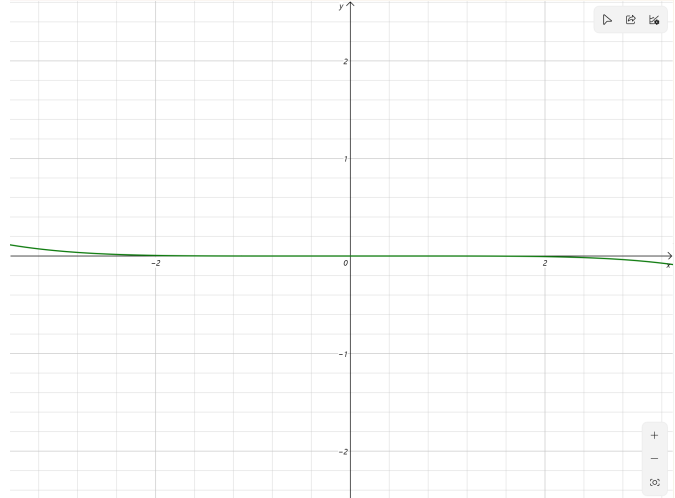
\includegraphics[width=0.8\textwidth]{hw2_20.png}\\
    \end{figure}
\par
均方误差:\par
$\Vert\delta\Vert_2^2 = \int_{-1}^{1}(f(x)-P(x))^{2} \mathrm{~d} x \approx 1.96709 \times 10^{-10}$
\paragraph{第22题}~{}
\\

$\Phi=\operatorname{span}\left\{1, x^{2}\right\}$ \par
\[
    \begin{array}{c}\left(\varphi_{0}, \varphi_{0}\right)=\sum\limits_{i=1}^{5} \varphi_{0}\left(x_{i}\right)^{2}=5, \quad\left(\varphi_{0}, \varphi_{1}\right)=\sum\limits_{i=1}^{5} \varphi_{0}\left(x_{i}\right) \varphi_{1}\left(x_{i}\right)=5327 \\ \left(\varphi_{1}, \varphi_{1}\right)=7277699, \quad\left(\varphi_{0}, y\right)=271.4, \quad\left(\varphi_{1}, y\right)=369321.5\end{array}    
\]\par
法方程为:\par
\begin{eqnarray}
    \left[\begin{array}{cc}5 & 5327 \\ 5327 & 7277699\end{array}\right]\left[\begin{array}{l}a \\ b\end{array}\right]=\left[\begin{array}{c}271.4 \\ 369321.5\end{array}\right]
\end{eqnarray}\par
解得: $a \approx 0.972748, b=0.050035$\par
所以经验公式:$y=0.972748+0.050035 x^{2}$\par
均方误差:$\Vert\delta\Vert_2^2=\sum_{i=1}^{5}\left(a+b x_{i}^{2}-y_{i}\right)^{2} \approx 0.015023$
\paragraph{第24题}~{}
\\

观察源数据的图像,可以发现$y$随着$t$单调递增,但是随着$t$越大,$y$的增长率越小,可以
得到$y^{'}>0, y^{''} <0$,可以建立拟合模型:$y=a \mathrm{e}^{-\frac{b}{t}}, a,b>0$\par
等式两边取对数:\par
$$\ln y=\ln a-\frac{b}{t} $$\par
令$\Phi=\operatorname{span}\left\{1,-\frac{1}{t}\right\}$\par
得到:\par
\begin{eqnarray}
    \begin{array}{c}(1,1)=\sum_{i=1}^{11} 1=11, \quad\left(1,-\frac{1}{t}\right)=-0.603975 \\ \left(-\frac{1}{t},-\frac{1}{t}\right)=0.062321, \quad(1, \ln y)=-87.674095, \quad\left(-\frac{1}{t}, \ln y\right)=5.032489\end{array}
\end{eqnarray}\par
法方程:\par
\begin{eqnarray}
    \left[\begin{array}{cc}11 & -0.603975 \\ -0.603975 & 0.062321\end{array}\right]\left[\begin{array}{c}{\ln a} \\ b\end{array}\right]=\left[\begin{array}{c}-87.674095 \\ 5.032489\end{array}\right]
\end{eqnarray}\par
解得:
$\ln a=-7.558781, b=7.4961692, a=5.215148 \times 10^{-4}$\par
$\therefore y=5.215148 \times 10^{-4} \times e^{-\frac{7.4961692}{t}}$

{\centering\section*{第四章}}

\paragraph{第1题}~{}
\\

\begin{enumerate}
    \item [(3)]
    为了使求积公式
    \begin{equation}
        \int_{-1}^{1} f(x) \mathrm{d} x \approx \frac{f(-1)+2 f\left(x_{1}\right)+3 f\left(x_{2}\right)}{3} \label{4.1}
    \end{equation}
    具有尽可能高的代数精度,只需取
    \begin{equation}
        f(x) = x^m, m=0, 1, 2, ...
    \end{equation}
    对\ref{4.1}式均准确成立即可\par
    当$f(x) = 1$时,$2 = \frac{1}{3}\left(1+2+3\right)$成立,所以\ref{4.1}准确成立. \par
    当$f(x) = x, f(x) = x^2$时,代入\ref{4.1}可得:\par
    \begin{equation}
        \left\{\begin{array}{l}-1+2 x_{1}+3 x_{2}=0 \\ 1+2 x_{1}^{2}+3 x_{2}^{2}=2\end{array}\right. 
    \end{equation}
    解得:
    \begin{equation}
        \left\{\begin{array}{l}x_{1}=-0.2898979 \\ x_{2}=0.6265986\end{array} \quad\right. \text{或}
    \quad\left\{\begin{array}{c}x_{1}=0.6898979 \\ x_{2}=-0.1265986\end{array}\right.
    \end{equation}
    若再将$f(x) = x^3$带入已经确定的求积公式,则:\par
    \begin{equation}
        \int_{-1}^{1} f(x) \mathrm{d} x \neq \frac{f(-1)+2 f\left(x_{1}\right)+3 f\left(x_{2}\right)}{3} 
    \end{equation}
    因此求积公式具有2次代数精度,求值节点:\par
    \begin{equation}
        \left\{\begin{array}{l}x_{1}=-0.2898979 \\ x_{2}=0.6265986\end{array} \quad\right. \text{或}
    \quad\left\{\begin{array}{c}x_{1}=0.6898979 \\ x_{2}=-0.1265986\end{array}\right.
    \end{equation}
\end{enumerate}

\paragraph{第2题}~{}
\\

\begin{enumerate}
    \item [(1)]
    使用复化梯形公式($h=\frac{1}{8}$): 
    \begin{equation}
        T_{8}=\frac{h}{2}\left[f(0)+2 \sum_{k=1}^{7} f\left(x_{k}\right)+f(1)\right]=0.1114024
    \end{equation}
    使用复化Simpson公式($h=\frac{1}{8}$): 
    \begin{equation}
        S_{8}  =\frac{h}{6}\left[f(0)+4 \sum_{k=0}^{7} f\left(x_{k+\frac{1}{2}}\right)+2 \sum_{k=1}^{7} f\left(x_{k}\right)+f(1)\right]  =0.1115718
    \end{equation}
\end{enumerate}

\paragraph{第7题}~{}
\\

设将区间分成n等份,则$h = \frac{b-a}{n}$由误差公式:
\begin{equation}
    |R|=\left|\frac{b-a}{12} h^{2} f^{\prime \prime}(\eta)\right| = \left|\frac{b-a}{12} \left(\frac{b-a}{n}\right)^{2} f^{\prime \prime}(\eta)\right| \leq \frac{(b-a)^{3}}{12 n^{2}} M<\varepsilon
\end{equation} \par
其中, $M=\max \limits_{a \leq x \leq b}\left|f^{\prime \prime}(x)\right|$ \par
解得: 
$$n>\sqrt{\frac{(b-a)^{3} M}{12 \varepsilon}}$$

\newpage
\paragraph{第11题}~{}

\begin{enumerate}
    \item [(1)]
    如下表,其中$T_0^{(k)}$中下标代表加速次数,上标代表二分次数。
    \begin{table}[h]
        \centering
        \caption{}
        \label{tab:my-table}
        \begin{tabular}{llllll}
        \hline
        k & $T_0^{(k)}$ & $T_1^{(k-1)}$ & $T_2^{(k-2)}$ & $T_3^{(k-3)}$ & $T_4^{(k-4)}$  \\ \hline
        0 &   1.3333333        &  &  &  &  \\
        1 &   1.1666667        & 1.1111111 &  &  &  \\
        2 &   1.1166667        & 1.1000000 & 1.0992593 &  &  \\
        3 &   1.1032107        & 1.0987253 & 1.0986403 & 1.0986305 &  \\
        4 &   1.0997677        & 1.0986200 & 1.0986130 & 1.0986126 & 1.0986125 \\
        \hline 
        \end{tabular}
        \end{table} \par
        取$I = 1.0986125$。
    \item [(2)]
    做变换:$y=t+2$,则当$y\in [1, 3]$时,$t \in [-1, 1]$.
    则:
    \begin{equation}
        \int_{1}^{3} \frac{\mathrm{d} y}{y}=\int_{-1}^{1} \frac{\mathrm{d} t}{t+2}  
    \end{equation}
    三点高斯公式:
    \begin{equation}
        \begin{aligned}
            \int_{1}^{3} \frac{\mathrm{d} y}{y}= & \int_{-1}^{1} \frac{\mathrm{d} t}{t+2} \\
            \approx & \frac{5}{9}f\left(-\frac{\sqrt{15}}{5}\right) + \frac{8}{9}f(0) + \frac{5}{9} f\left(\frac{\sqrt{15}}{5}\right) \\
            \approx & 0.5555556\left(\frac{1}{2-0.7745967}+\frac{1}{2+0.7745967}\right) \\ & +0.8888889 \times \frac{1}{2+0}\\ 
            =& 1.0980393
        \end{aligned}
    \end{equation}
    五点高斯公式:
    \begin{equation}
        \begin{aligned} \int_{1}^{3} \frac{\mathrm{d} y}{y}= & \int_{-1}^{1} \frac{\mathrm{d} t}{t+2} \approx 0.2369269 \\ & \left(\frac{1}{2-0.9061798}+\frac{1}{2+0.9061798}\right) \\ & +0.4786289\left(\frac{1}{2-0.5384693}+\frac{1}{2+0.5384693}\right) \\ & +0.5688889 \times \frac{1}{2+0}=1.0986093\end{aligned}
    \end{equation}
    \item [(3)]
    将区间$[1, 3]$分成四个小区间$[1, 1.5], [1.5, 2], [2, 2.5], [2.5, 3]$ \\
    在第一个区间上, 做变换$y = \frac{1}{4}t + \frac{5}{4}$.
    \begin{equation}
        \begin{aligned} I_{1} & =\int_{1}^{1.5} \frac{\mathrm{d} y}{y}=\int_{-1}^{1} \frac{1 \mathrm{~d} t}{5+ t} \\ & \approx 0.5 \times\left[\frac{1}{2.5+0.5 \times\left(-\frac{1}{\sqrt{3}}\right)}+\frac{1}{2.5+0.5 \times\left(\frac{1}{\sqrt{3}}\right)}\right] \\ & =0.4054054\end{aligned}
    \end{equation}
    在第二个区间上, 做变换$y = \frac{1}{4}t + \frac{7}{4}$.
    \begin{equation}
        \begin{aligned}
            I_{2} &=\int_{1.5}^{2} \frac{\mathrm{d} y}{y}=\int_{-1}^{1} \frac{1 \mathrm{~d} t}{7+ t} \\
            & \approx 0.5 \times\left[\frac{1}{3.5+0.5 \times\left(-\frac{1}{\sqrt{3}}\right)}+\frac{1}{3.5+0.5 \times\left(\frac{1}{\sqrt{3}}\right)}\right] \\
            & =0.2876712
        \end{aligned}
    \end{equation}
    在第三个区间上, 做变换$y = \frac{1}{4}t + \frac{9}{4}$.
    \begin{equation}
        \begin{aligned} I_{3} & =\int_{2}^{2.5} \frac{\mathrm{d} x}{y}=\int_{-1}^{1} \frac{1 \mathrm{~d} t}{9+ t} \\ & \approx 0.5 \times\left[\frac{1}{4.5+0.5 \times\left(-\frac{1}{\sqrt{3}}\right)}+\frac{1}{4.5+0.5 \times\left(\frac{1}{\sqrt{3}}\right)}\right] \\ & =0.2231405\end{aligned}
    \end{equation}
    在第四个区间上, 做变换$y = \frac{1}{4}t + \frac{11}{4}$.
    \begin{equation}
        \begin{aligned} I_{4} & =\int_{2.5}^{3} \frac{\mathrm{d} y}{y}=\int_{-1}^{1} \frac{1 \mathrm{~d} t}{11+ t} \\ & \approx 0.5 \times\left[\frac{1}{5.5+0.5 \times\left(-\frac{1}{\sqrt{3}}\right)}+\frac{1}{5.5+0.5 \times\left(\frac{1}{\sqrt{3}}\right)}\right]\\ &=0.1823204\end{aligned}
    \end{equation}
    故:
    \begin{equation}
        I=I_{1}+I_{2}+I_{3}+I_{4} \approx 1.0985375
    \end{equation}
    \textbf{比较} \\
    积分真值:
    \begin{equation}
        I=\int_{1}^{3} \frac{\mathrm{d} y}{y}=\ln 3=1.098612288 \cdots
    \end{equation}
    说明龙贝格算法比高斯求积算法更准确,但龙贝格算法运算量更大。
\end{enumerate}
\end{document}
